% Created by tikzDevice version 0.12 on 2019-06-03 03:31:47
% !TEX encoding = UTF-8 Unicode
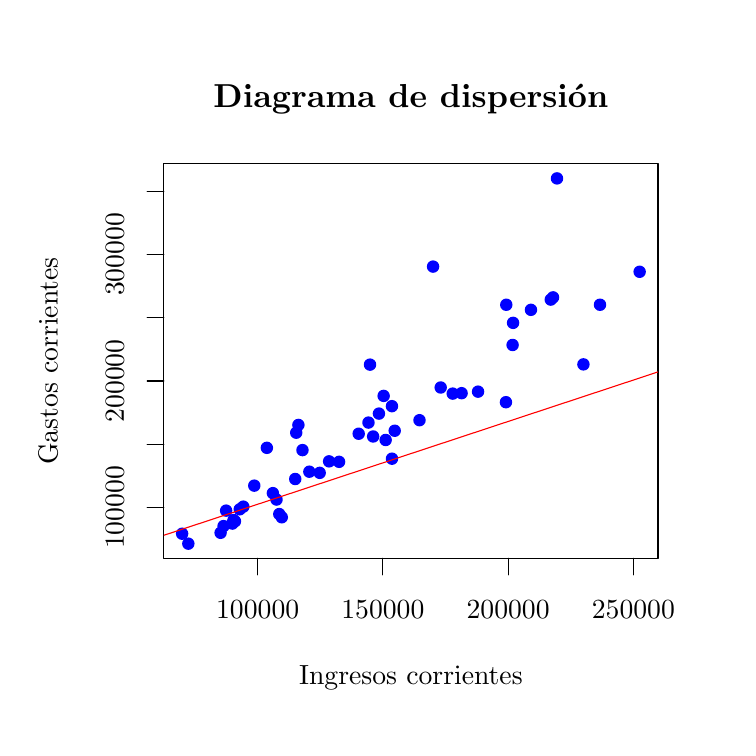
\begin{tikzpicture}[x=1pt,y=1pt]
\definecolor{fillColor}{RGB}{255,255,255}
\path[use as bounding box,fill=fillColor,fill opacity=0.00] (0,0) rectangle (252.94,252.94);
\begin{scope}
\path[clip] ( 49.20, 61.20) rectangle (227.75,203.75);
\definecolor{fillColor}{RGB}{0,0,255}

\path[fill=fillColor] ( 69.71, 70.41) circle (  2.25);

\path[fill=fillColor] ( 58.05, 66.48) circle (  2.25);

\path[fill=fillColor] ( 55.81, 70.08) circle (  2.25);

\path[fill=fillColor] ( 70.78, 72.83) circle (  2.25);

\path[fill=fillColor] ( 73.96, 73.74) circle (  2.25);

\path[fill=fillColor] ( 88.60, 84.75) circle (  2.25);

\path[fill=fillColor] ( 90.91, 77.18) circle (  2.25);

\path[fill=fillColor] ( 74.90, 74.56) circle (  2.25);

\path[fill=fillColor] ( 76.63, 78.91) circle (  2.25);

\path[fill=fillColor] ( 77.92, 79.86) circle (  2.25);

\path[fill=fillColor] ( 71.71, 78.43) circle (  2.25);

\path[fill=fillColor] ( 86.43,101.11) circle (  2.25);

\path[fill=fillColor] ( 91.82, 76.02) circle (  2.25);

\path[fill=fillColor] ( 74.39, 75.03) circle (  2.25);

\path[fill=fillColor] ( 81.88, 87.45) circle (  2.25);

\path[fill=fillColor] ( 89.92, 82.42) circle (  2.25);

\path[fill=fillColor] (105.52, 92.07) circle (  2.25);

\path[fill=fillColor] ( 97.83,109.38) circle (  2.25);

\path[fill=fillColor] (108.92, 96.23) circle (  2.25);

\path[fill=fillColor] ( 96.68, 89.85) circle (  2.25);

\path[fill=fillColor] ( 99.30,100.30) circle (  2.25);

\path[fill=fillColor] ( 97.04,106.58) circle (  2.25);

\path[fill=fillColor] (112.52, 96.06) circle (  2.25);

\path[fill=fillColor] (189.02,154.68) circle (  2.25);

\path[fill=fillColor] (131.64, 97.19) circle (  2.25);

\path[fill=fillColor] (101.78, 92.49) circle (  2.25);

\path[fill=fillColor] (124.83,105.21) circle (  2.25);

\path[fill=fillColor] (123.15,110.24) circle (  2.25);

\path[fill=fillColor] (119.61,106.21) circle (  2.25);

\path[fill=fillColor] (123.70,131.18) circle (  2.25);

\path[fill=fillColor] (141.58,111.10) circle (  2.25);

\path[fill=fillColor] (129.36,103.95) circle (  2.25);

\path[fill=fillColor] (126.93,113.48) circle (  2.25);

\path[fill=fillColor] (128.63,119.88) circle (  2.25);

\path[fill=fillColor] (131.63,116.17) circle (  2.25);

\path[fill=fillColor] (146.49,166.60) circle (  2.25);

\path[fill=fillColor] (156.80,120.86) circle (  2.25);

\path[fill=fillColor] (132.63,107.29) circle (  2.25);

\path[fill=fillColor] (153.59,120.71) circle (  2.25);

\path[fill=fillColor] (149.25,122.91) circle (  2.25);

\path[fill=fillColor] (162.74,121.41) circle (  2.25);

\path[fill=fillColor] (172.94,152.81) circle (  2.25);

\path[fill=fillColor] (175.40,146.27) circle (  2.25);

\path[fill=fillColor] (172.82,117.60) circle (  2.25);

\path[fill=fillColor] (175.23,138.28) circle (  2.25);

\path[fill=fillColor] (189.84,155.48) circle (  2.25);

\path[fill=fillColor] (181.86,150.98) circle (  2.25);

\path[fill=fillColor] (191.27,198.47) circle (  2.25);

\path[fill=fillColor] (221.13,164.73) circle (  2.25);

\path[fill=fillColor] (200.82,131.27) circle (  2.25);

\path[fill=fillColor] (206.81,152.82) circle (  2.25);
\end{scope}
\begin{scope}
\path[clip] (  0.00,  0.00) rectangle (252.94,252.94);
\definecolor{drawColor}{RGB}{0,0,0}

\path[draw=drawColor,line width= 0.4pt,line join=round,line cap=round] ( 83.11, 61.20) -- (218.87, 61.20);

\path[draw=drawColor,line width= 0.4pt,line join=round,line cap=round] ( 83.11, 61.20) -- ( 83.11, 55.20);

\path[draw=drawColor,line width= 0.4pt,line join=round,line cap=round] (128.36, 61.20) -- (128.36, 55.20);

\path[draw=drawColor,line width= 0.4pt,line join=round,line cap=round] (173.62, 61.20) -- (173.62, 55.20);

\path[draw=drawColor,line width= 0.4pt,line join=round,line cap=round] (218.87, 61.20) -- (218.87, 55.20);

\node[text=drawColor,anchor=base,inner sep=0pt, outer sep=0pt, scale=  1.00] at ( 83.11, 39.60) {100000};

\node[text=drawColor,anchor=base,inner sep=0pt, outer sep=0pt, scale=  1.00] at (128.36, 39.60) {150000};

\node[text=drawColor,anchor=base,inner sep=0pt, outer sep=0pt, scale=  1.00] at (173.62, 39.60) {200000};

\node[text=drawColor,anchor=base,inner sep=0pt, outer sep=0pt, scale=  1.00] at (218.87, 39.60) {250000};

\path[draw=drawColor,line width= 0.4pt,line join=round,line cap=round] ( 49.20, 79.59) -- ( 49.20,193.83);

\path[draw=drawColor,line width= 0.4pt,line join=round,line cap=round] ( 49.20, 79.59) -- ( 43.20, 79.59);

\path[draw=drawColor,line width= 0.4pt,line join=round,line cap=round] ( 49.20,102.44) -- ( 43.20,102.44);

\path[draw=drawColor,line width= 0.4pt,line join=round,line cap=round] ( 49.20,125.28) -- ( 43.20,125.28);

\path[draw=drawColor,line width= 0.4pt,line join=round,line cap=round] ( 49.20,148.13) -- ( 43.20,148.13);

\path[draw=drawColor,line width= 0.4pt,line join=round,line cap=round] ( 49.20,170.98) -- ( 43.20,170.98);

\path[draw=drawColor,line width= 0.4pt,line join=round,line cap=round] ( 49.20,193.83) -- ( 43.20,193.83);

\node[text=drawColor,rotate= 90.00,anchor=base,inner sep=0pt, outer sep=0pt, scale=  1.00] at ( 34.80, 79.59) {100000};

\node[text=drawColor,rotate= 90.00,anchor=base,inner sep=0pt, outer sep=0pt, scale=  1.00] at ( 34.80,125.28) {200000};

\node[text=drawColor,rotate= 90.00,anchor=base,inner sep=0pt, outer sep=0pt, scale=  1.00] at ( 34.80,170.98) {300000};

\path[draw=drawColor,line width= 0.4pt,line join=round,line cap=round] ( 49.20, 61.20) --
	(227.75, 61.20) --
	(227.75,203.75) --
	( 49.20,203.75) --
	( 49.20, 61.20);
\end{scope}
\begin{scope}
\path[clip] (  0.00,  0.00) rectangle (252.94,252.94);
\definecolor{drawColor}{RGB}{0,0,0}

\node[text=drawColor,anchor=base,inner sep=0pt, outer sep=0pt, scale=  1.20] at (138.47,224.20) {\bfseries Diagrama de dispersión};

\node[text=drawColor,anchor=base,inner sep=0pt, outer sep=0pt, scale=  1.00] at (138.47, 15.60) {Ingresos corrientes};

\node[text=drawColor,rotate= 90.00,anchor=base,inner sep=0pt, outer sep=0pt, scale=  1.00] at ( 10.80,132.47) {Gastos corrientes};
\end{scope}
\begin{scope}
\path[clip] ( 49.20, 61.20) rectangle (227.75,203.75);
\definecolor{drawColor}{RGB}{255,0,0}

\path[draw=drawColor,line width= 0.4pt,line join=round,line cap=round] ( 49.20, 69.51) -- (227.75,128.54);
\end{scope}
\end{tikzpicture}
